\documentclass[conference]{IEEEtran}
\usepackage{cite}
\usepackage{graphicx}
\usepackage{placeins}
\usepackage{caption}
\usepackage{subfigure}
\usepackage{enumerate}
\usepackage{afterpage}
\usepackage[font={small}]{caption}
\AtBeginDocument{\renewcommand{\abstractname}{Resumo}}
\begin{document}
\title{Projeto 2 de Princ\'ipios de Vis\~ao Computacional}
\author{\IEEEauthorblockN{Gabriel Martins de Miranda}
\IEEEauthorblockA{130111350\\
Universidade de Bras\'ilia\\
Email:gabrielmirandat@hotmail.com}
}
\maketitle
\begin{abstract}
A presente demonstra\c{c}\~ao se baseia no algoritmo de M.Brown e D.Lowe, implemetados na classe inv\'olucro image stitching.
Dado um conjunto de imagens da torre de tv de bras\'ilia, tiradas apenas rotacionando a c\^amera num eixo fixo em 
180 graus, criou-se um panorama robusto, invariante a ordem das imagens de entrada, orienta\c{c}\~ao, escala e ilumina\c{c}\~ao.
\end{abstract}

\section{ Introdu\c{c}\~ao} 
\label{sec:meth} 
	Um panorama caracteriza-se pelo concatenac{c}\~ao de algumas/v\'arias imagens de forma que dada esta uni\~ao tem-se
	uma vis\~ao mais ampla do que com cada imagem em separado.
	
	De uma maneira geral, para se criar uma imagem panor\^amica simples, realizamos os seguintes passos:
	\\
\begin{enumerate}
	\item Tirar sequ\^encia de fotos a partir da mesma posi\c{c}\~ao, rotacionando a c\^amera sobre seu eixo \'optico.
	\item Computar a transforma\c{c}\~ao T da segunda para a primeira imagem.
	\item Moldar a segunda imagem para se sobrepor \`a primeira.
	\item Repetir para todas as outras.
\end{enumerate}

Acontece que com esta abordagem, n\~ao conseguimos obter um panorama t\~ao robusto e invariante como o proposto
neste projeto demonstrativo.

Uma abordagem mais convincente foi proposta e j\'a vem implementada no m\'odulo $stitching.\> Images$ $stitching$, presente
no software OpenCV. De maneira geral, segue os passos utilizados pelo m\'odulo:
  \\
\begin{enumerate}  
  \item Encontrar features invariantes.
  \item Eliminar features desnecess\'arias.
  \item Encontrar relacionamento entre todas as imagens atrav\'es do casamento de features comuns (vetores descritores).
  \item Relizar casamentos para constru\c{c}\~ao do panorama propriamente dito.
  \item Retificar efeito ondulado do panorama.
  \item Otimizar o resultado homogeneizando \'areas pr\'oximas e eliminando o efeito de costura.

\end{enumerate}	 
     
\section{Metodologia} 
\label{sec:meth} 
     
     O primeiro passo no algoritmo do panorama \'e encontrar caracter\'isticas que possam definir/diferenciar uma imagem de 
     outra. Estas caracter\'isticas, chamadas de $features$, geralmente s\~ao cantos retirados do cruzamento entre duas bordas.
     
     Abordagens tradicionais para localiza\c{c}\~ao de cantos, tais como o de $Harris$, apesar de serem algoritmos robustos, 
     caem em um dos problemas de invari\^ancia. No caso de $Harris$, mudan\c{c}as
     na escala podem impedir a localiza\c{c}\~ao destas caracter\'isticas.
     
     Atra\'ves do algoritmo $Scale$ $Invariant$ $Feature$ $Transform$, $SIFT$, \'e poss\'ivel obter $features$ invariantes.
     Estas est\~ao localizadas na rela\c{c}\~ao escala-espacial de diferen\c{c}a m\'axima/m\'inima da fun\c{c}\~ao Gaussiana.
     Em cada localiza\c{c}\~ao de $feature$, caracter\'isticas de escala e orienta\c{c}\~ao s\~ao estabelecidas. Isto nos d\'a
     um quadro de similaridade-invari\^ancia no qual podemos fazer medidas. O m\'etodo ent\~ao realiza o histograma das orienta\c{c}\~oes
     dos gradientes locais. Este acumulo espacial \'e muito importante para a invari\^ancia do SHIFT.
     
     Isto permite que as bordas se desloquem sem alterar os vetores descritores (aqueles que indicam o relacionanto entre
     features comuns nas diferentes imagens que comp\~oem o panorama), dando grande robustez para as posteriores transforma\c{c}\~oes
     afins.
     
     A invari\^ancia \`a ilumina\c{c}\~ao \'e adquirida pelo uso de gradientes e pela normaliza\c{c}\~ao dos vetores descritores.
  
    Uma vez que as $features$ foram extra\'idas de todas as imagens, elas devem ser relacionadas umas com as outras. Cada $feature$ 
    \'e casada com seus k vizinhos mais pr\'oximos em seu espa\c{c}o de atua\c{c}\~ao, atrav\'es do algoritmo $k-d\>tree$.
  
  O segundo passo se trata do descarte de features desnecess\'arias e do casamento das imagens, que futuramente se tornar\~ao
  um panorama. Do passo anterior, n\'os identificamos imagens que tem um grande n\'umero de $matches$ entre si. Consideramos um n\'umero
  fixo de $m$ imagens que possuem os maiores n\'umeros de casamentos de features com a imagem atual, como potenciais para 
  a concatena\c{c}\~ao entre elas. Primeiro, usamos o m\'etodo $RANdom$ $SAmple$ $Consensus$, $RANSAC$, para selecionar
  um conjunto de $inliers$, (ou features boas, contidas num intervalo de m\'inimo-m\'aximo numa reta de transi\c{c}\~ao) que
  s\~ao compat\'iveis com uma homografia entre as imagens. Os outliers (features ruins, ou que ficaram fora do intervalo)
  s\~ao descartados. Depois disto, aplicamos um m\'etodo probabil\'istico para verificar o match.
  
  O descarte proposto pelo $RANSAC$ \'e muito importante pois diminui muito a complexidade e custo de processamento, 
  permitindo r\'apida estima\c{c}\~ao das matrizes de homografia entre as imagens que possuem correspond\^encia atrav\'es
  dos inliers encontrados. Desta maneira, as imagens s\~ao alinhadas e unidas de acordo com a homografia encontrada.
  
  Os passos seguidos at\'e ent\~ao nos d\'a a rota\c{c}\~ao relativa entre as imagens, mas n\~ao permite saber como s\~ao
  no mundo 3D. Se simplesmente assumirmos que R (rota\c{c}\~ao) = I (identidade) para uma das imagens, tipicamente nos deparamos 
  com um efeito onludalado na sa\'ida do panorama. Podemos corrigir esta ondula\c{c}\~ao usando a heur\'istica do modo 
  como as pessoas geralmente tiram fotos panor\^amicas. \'E raro as pessoas torcerem a c\^amera relativamente ao horizonte, 
  ent\~ao os vetores horizontais da c\^amera recaem num plano comum. Assim \'e poss\'ivel corrigir este efeito aplicando
  uma rota\c{c}\~ao global derivada desta suposi\c{c}\~ao.
  
  Atrav\'es dos par\^ametros geom\'etricos da c\^amera, (orienta\c{c}\~ao e dist\^ancia focal), podemos encontrar um 
  par\^ametro fotom\'etrico, o ganho geral entre as imagens. Atrav\'es deste ganho global e do uso do algoritmo de Burt
  e Adelson chamado $multi-band$ $blending$, que suaviza as intensidades de pixels diferentes entre $features$ iguais (que 
  foram correspondidas na sa\'ida do panorama), podemos realizar um acabamento e otimizar o resultado final do panorama.
  
  Diante destes passos, pode-se simular uma situ\c{c}\~ao fict\'icia de como o algoritmo de obten\c{c}\~ao de panoramas funciona:
  \\\\
  Assumindo que se quer unir 4 imagens, $I_{0},\>I_{1},\>I_{2},\>I_{3}$, o objetivo \'e computar as matrizes de homografia
  $H_{0},\>H_{1},\>H_{2},\>H_{3}$.

\begin{enumerate}
	\item Computar todos os pares de homografias $H_{01},\>H_{02},\>H_{03},\>H_{12},\>H_{13},\>H_{23}$, onde homografia 
	 $H_{01} $ molda a imagem $I_{0}$ na $I_{1}$, etc.
	\item Selecionar uma imagem \^ancora, por exemplo $I_{1}$ cuja posi\c{c}\~ao ficar\'a fixa. Para isto, podemos escolher
	 $H_{1}$ como sendo a matriz identidade.
	\item Encontrar imagem que melhor se alinha com $I_{1}$ baseado no n\'umero m\'aximo de $matches$ consistentes, por
	 exemplo $I_{3}$.
	 \item Atualizar $H_{3}\>=\>H_{1}$x$H_{13}^{-1}\>=\>H_{13}^{-1}\>=\>H_{31}$
	 \item Encontrar imagem que melhor se encaixe com $I_{1}$ ou $I_{3}$, por exemplo $I_{2}$ em $I_{3}$.
	 \item Atualizar $H_{2}\>=\>H_{3}$x$H_{23}$
	 \item Idem para $I_{0}$
	 \item Fazer ajuste para otimizar o alinhamento global.
	 
\end{enumerate}	

\section{Resultados} 
\label{sec:meth} 
1) Imagens tiradas de cima da torre de TV(c\^amera rotacionando s\'o na horizontal):

		\vspace{2\baselineskip}\vspace{-\parskip}
		\begin{minipage}{\linewidth}
  		\centering
  		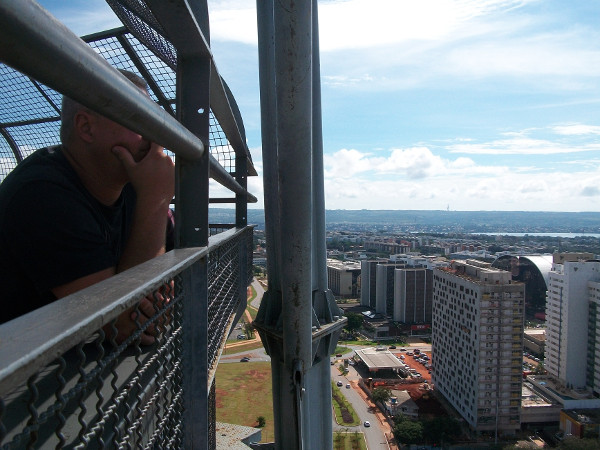
\includegraphics[width=3.3in]{t1}
  		\captionof{figure}{imagem 1/6. Vista em cima da torre.}
		\end{minipage}
		
		\vspace{2\baselineskip}\vspace{-\parskip}
		\begin{minipage}{\linewidth}
  		\centering
  		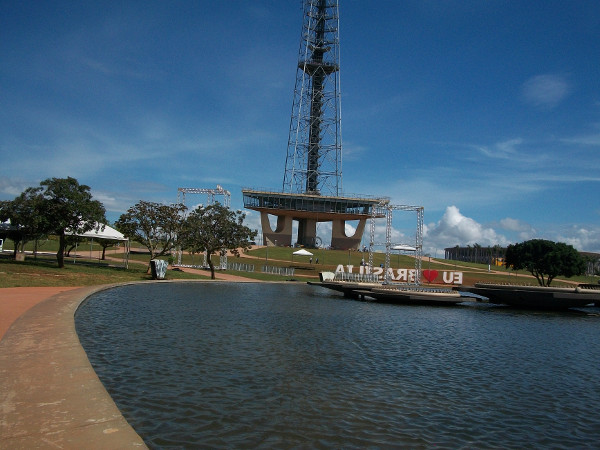
\includegraphics[width=3.3in]{t2}
  		\captionof{figure}{imagem 2/6. Vista em cima da torre.}
		\end{minipage}
		
		\vspace{2\baselineskip}\vspace{-\parskip}
		\begin{minipage}{\linewidth}
  		\centering
  		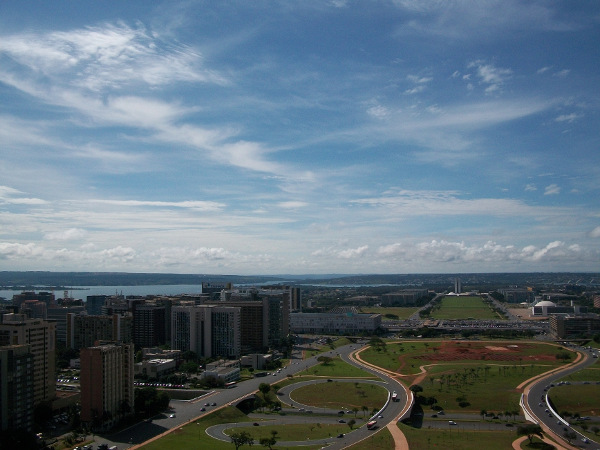
\includegraphics[width=3.3in]{t3}
  		\captionof{figure}{imagem 3/6. Vista em cima da torre.}
		\end{minipage}
		
		\vspace{2\baselineskip}\vspace{-\parskip}
		\begin{minipage}{\linewidth}
  		\centering
  		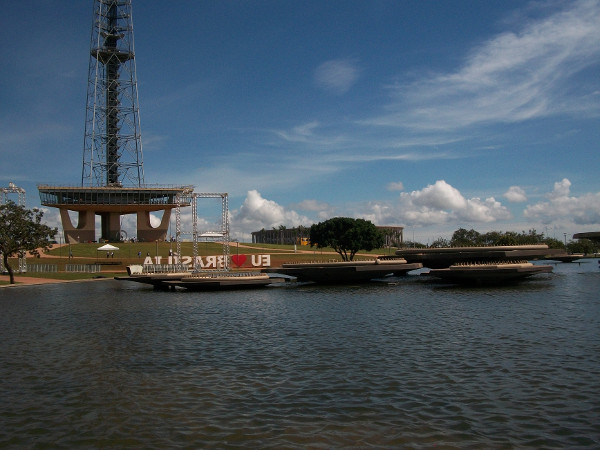
\includegraphics[width=3.3in]{t4}
  		\captionof{figure}{imagem 4/6. Vista em cima da torre.}
		\end{minipage}
		
		\vspace{2\baselineskip}\vspace{-\parskip}
		\begin{minipage}{\linewidth}
  		\centering
  		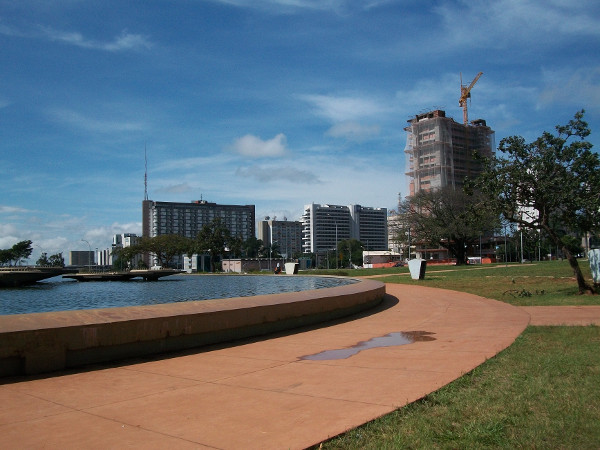
\includegraphics[width=3.3in]{t5}
  		\captionof{figure}{imagem 5/6. Vista em cima da torre.}
		\end{minipage}
		
		\vspace{2\baselineskip}\vspace{-\parskip}
		\begin{minipage}{\linewidth}
  		\centering
  		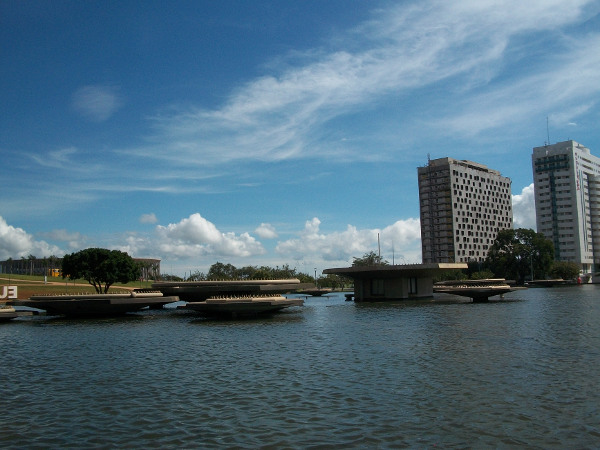
\includegraphics[width=3.3in]{t6}
  		\captionof{figure}{imagem 6/6. Vista em cima da torre.}
		\end{minipage}


2) Imagens tiradas de baixo da torre de TV(c\^amera rotacionando na horizontal e vertical):

		\vspace{2\baselineskip}\vspace{-\parskip}
		\begin{minipage}{\linewidth}
  		\centering
  		\includegraphics[width=3.3in]{t15}
  		\captionof{figure}{imagem 1/14. Vista em baixo da torre.}
		\end{minipage}
		
		\vspace{2\baselineskip}\vspace{-\parskip}
		\begin{minipage}{\linewidth}
  		\centering
  		\includegraphics[width=3.3in]{t25}
  		\captionof{figure}{imagem 2/14. Vista em baixo da torre.}
		\end{minipage}
		
		\vspace{2\baselineskip}\vspace{-\parskip}
		\begin{minipage}{\linewidth}
  		\centering
  		\includegraphics[width=3.3in]{t45}
  		\captionof{figure}{imagem 4/14. Vista em baixo da torre.}
		\end{minipage}
		
		\vspace{2\baselineskip}\vspace{-\parskip}
		\begin{minipage}{\linewidth}
  		\centering
  		\includegraphics[width=3.3in]{t75}
  		\captionof{figure}{imagem 7/14. Vista em baixo da torre.}
		\end{minipage}
		
		\vspace{2\baselineskip}\vspace{-\parskip}
		\begin{minipage}{\linewidth}
  		\centering
  		\includegraphics[width=3.3in]{t105}
  		\captionof{figure}{imagem 10/14. Vista em baixo da torre.}
		\end{minipage}
		
		\vspace{2\baselineskip}\vspace{-\parskip}
		\begin{minipage}{\linewidth}
  		\centering
  		\includegraphics[width=3.3in]{t115}
  		\captionof{figure}{imagem 11/14. Vista em baixo da torre.}
		\end{minipage}
		
		\vspace{2\baselineskip}\vspace{-\parskip}
		\begin{minipage}{\linewidth}
  		\centering
  		\includegraphics[width=3.3in]{t125}
  		\captionof{figure}{imagem 12/14. Vista em baixo da torre.}
		\end{minipage}
		
		\vspace{2\baselineskip}\vspace{-\parskip}
		\begin{minipage}{\linewidth}
  		\centering
  		\includegraphics[width=3.3in]{t135}
  		\captionof{figure}{imagem 13/14. Vista em baixo da torre.}
		\end{minipage}

		\vspace{2\baselineskip}\vspace{-\parskip}
		\begin{minipage}{\linewidth}
  		\centering
  		\includegraphics[width=3.3in]{t145}
  		\captionof{figure}{imagem 14/14. Vista em baixo da torre.}
		\end{minipage}		 	

	
		
		\vspace{2\baselineskip}\vspace{-\parskip}
		\begin{minipage}{\linewidth}
  		\centering
  		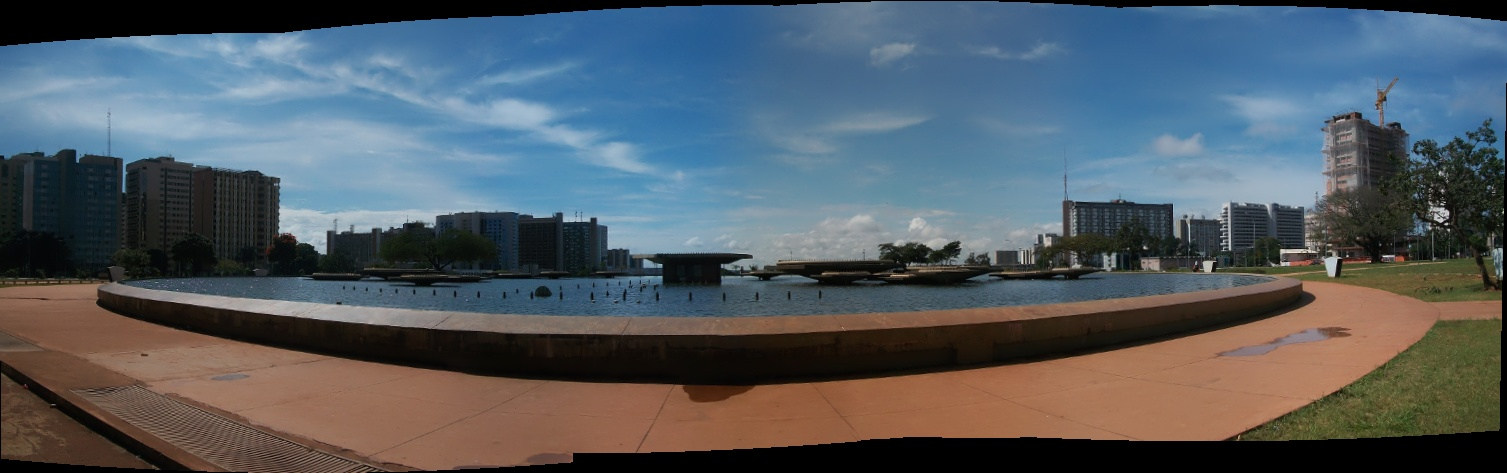
\includegraphics[width=7.0 in]{final}
  		\captionof{figure}{imagem resultado. Vista em cima da torre.}
		\end{minipage}
	
		
		\vspace{2\baselineskip}\vspace{-\parskip}
		\begin{minipage}{\linewidth}
  		\centering
  		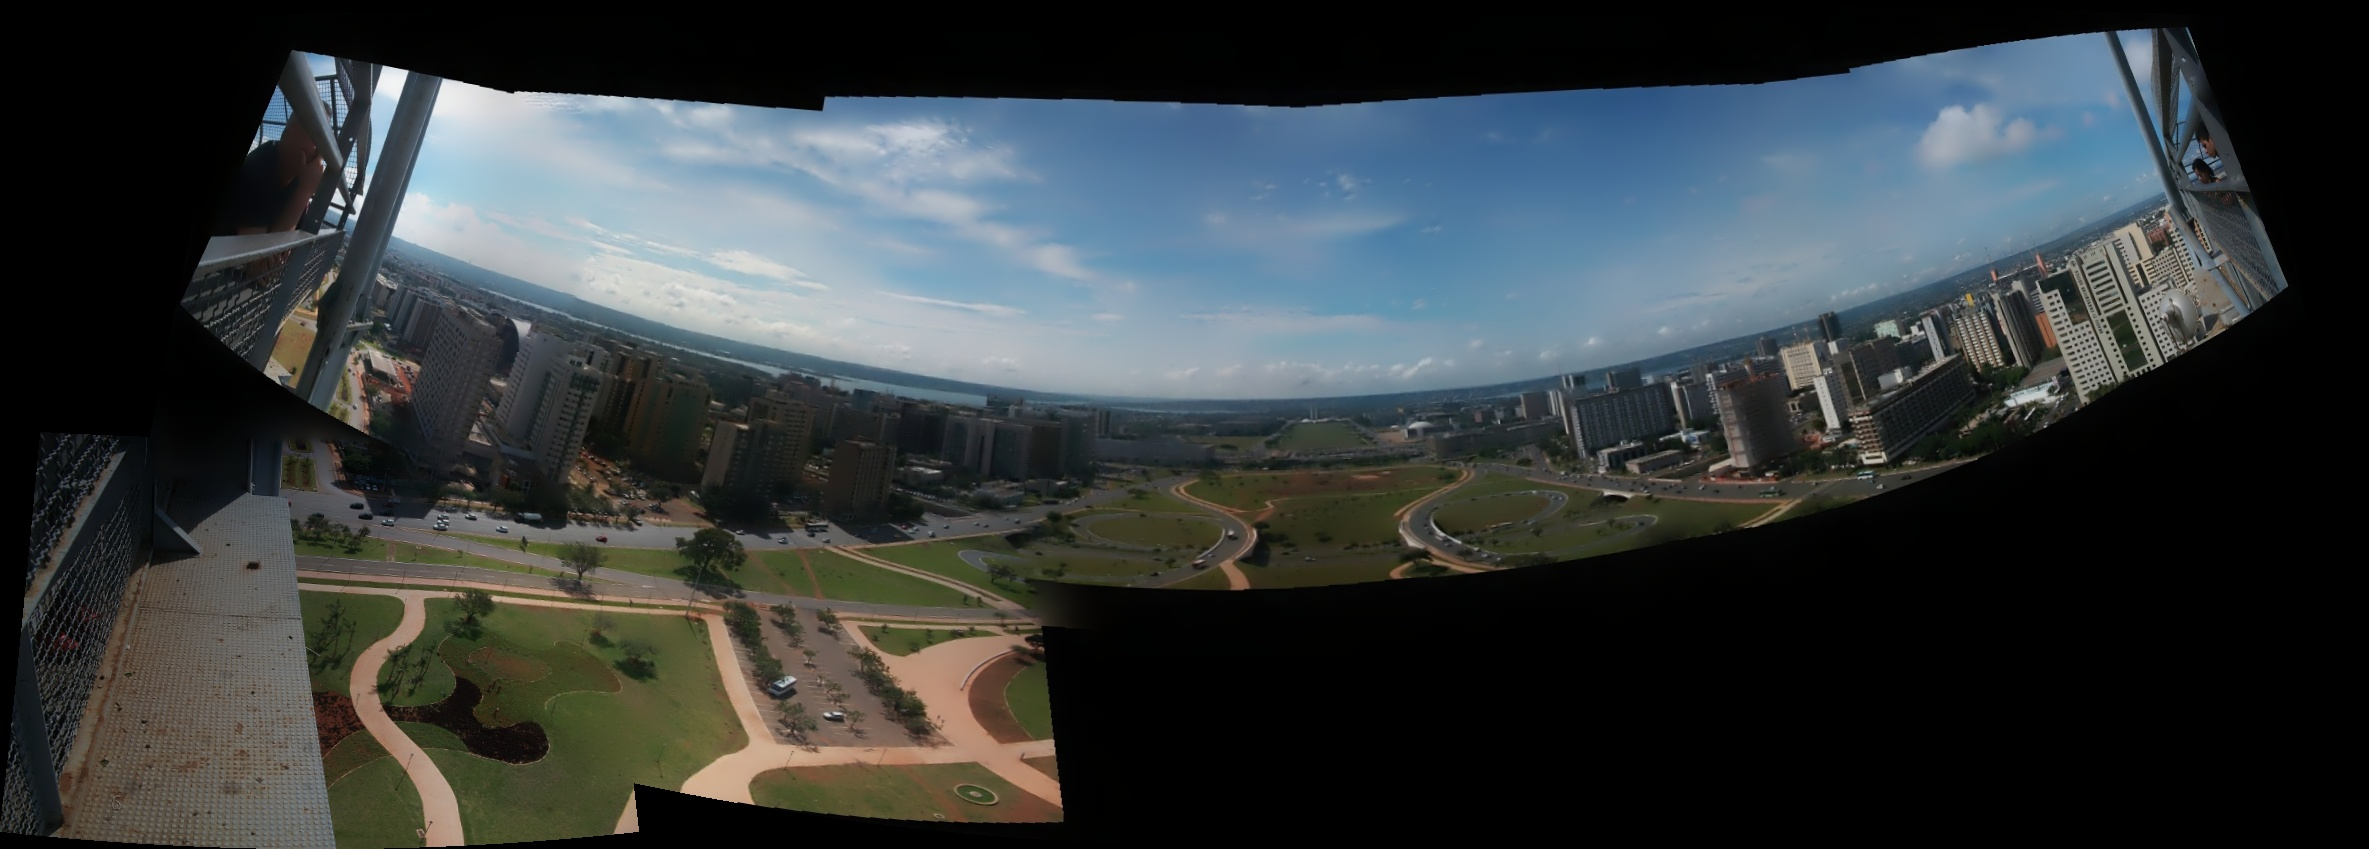
\includegraphics[width=7.0 in]{final2}
  		\captionof{figure}{imagem resultado. Vista em baixo da torre.}
		\end{minipage}	
	
	
\section{Conclus\~ao} 
\label{sec:meth} 

Atrav\'es do algoritmo aqui proposto, torna-se poss\'ivel a cria\c{c}\~ao de panoramas robustos e invariantes \`a quest\~oes
referentes \`a escala, zoom, ilumina\c{c}\~ao e orienta\c{c}\~ao. Os resultados s\~ao surpreentes, gra\c{c}as  as etapas de
otimiza\c{c}\~ao, torna-se dif\'icil supor que houve jun\c{c}\~ao de imagens, j\'a que n\~ao se pode ver as bordas das imagens
 que comp\~oem o panorama.

\section{Refer\^encias} 
\label{sec:meth} 

[1] Automatic Panoramic Image Stitching using Invariant Features, Matthew Brown and David G. Lowe.

[2] Eric Yuan's Blog Perstando et Praestando RANSAC.

[3] ramsrigoutham A wayfarer's monologue! Panorama – Image Stitching in OpenCV

[4] Project4: Image Warping and Mosaicing Danielle Millett

[5]  OpenCV Stitching example (Stitcher class, Panorama) - MARE's Computer Vision Study
\end{document}